\documentclass{article}
\usepackage{tikz}

\begin{document}

\begin{tikzpicture}[scale=1.5]
    % Define coordinates for nodes
    \foreach \i in {1,...,\alpha} {
        \node[draw] (a\i) at (\i, 0) {\(\alpha + \i\beta\)};
    }
    \foreach \i in {1,...,2} {
        \node[draw] (b\i) at (-3, \i) {\(\i\)};
    }
    \node[draw] (c) at (3, 0) {\(\alpha + \alpha\beta + 1\)};
    
    % Draw edges
    \foreach \i in {1,...,\alpha} {
        \foreach \j in {1,2} {
            \draw (a\i) -- (b\j);
        }
    }
    \foreach \i in {1,...,2} {
        \draw (b\i) -- (c);
    }
    
    % Add labels for specific nodes
    \node[above] at (a1) {\(\alpha + \beta\)};
    \node[above] at (a2) {\(\alpha + \beta + 1\)};
    \node[above] at (a3) {\(\alpha + \beta + 2\)};
    \node[above] at (a4) {\(\alpha + (\alpha - 1)\beta + 1\)};
    \node[above] at (a5) {\(\alpha + (\alpha - 1)\beta + 2\)};
    \node[above] at (a6) {\(\alpha + \alpha\beta\)};
    
    % Dotted lines
    \draw[dotted] (a1) -- (a6);
    \draw[dotted] (a2) -- (a5);
    \draw[dotted] (a3) -- (a4);
    
    % Labels for nodes b
    \node[left] at (b1) {\(1\)};
    \node[left] at (b2) {\(2\)};
    
    % Label for node c
    \node[right] at (c) {\(\alpha + \alpha\beta + 2\)};
\end{tikzpicture}

\end{document}